\documentclass[11pt]{article}

\usepackage[margin=1in]{geometry}
\usepackage{amsmath, amssymb}
\usepackage{physics}
\usepackage{graphicx}
\usepackage{booktabs}
\usepackage{siunitx}
\usepackage{xcolor}
\usepackage[colorlinks=true, linkcolor=blue, urlcolor=blue]{hyperref}

\newcommand{\kT}{k_{B}T}
\newcommand{\kbond}{k_{\mathrm{bond}}}
\newcommand{\rzero}{r_{0}}
\newcommand{\avg}[1]{\left\langle #1 \right\rangle}

\title{Equilibrium Bond--Length Distribution of a Harmonic Dumbbell\\
\large Why the mean bond length exceeds the rest length}
\author{PolyStokes --- Brownian dynamics notes}
\date{\today}

\begin{document}
\maketitle

\begin{abstract}
For two beads joined by a harmonic spring in three dimensions, the equilibrium
probability density of the \emph{scalar} bond length carries a geometric factor
$r^{2}$ that is absent from the Boltzmann weight of the bond \emph{vector}. As a
result the mean bond length sits \emph{above} the rest length $\rzero$, and for a
soft spring ($\kbond\,\rzero^{2}\ll \kT$) the deviation is large and set by the
thermal width $\sigma=\sqrt{\kT/\kbond}$ rather than by $\rzero$. This note derives
the distribution, evaluates its mean exactly through a truncated--Gaussian moment
recurrence, and connects the result to the purely--thermal dumbbell simulation.
\end{abstract}

\section{Setup}

Two beads at positions $\vb{x}_{1},\vb{x}_{2}\in\mathbb{R}^{3}$ are joined by a
harmonic bond that depends only on the length $r=\abs{\vb{b}}$ of the bond vector
$\vb{b}=\vb{x}_{2}-\vb{x}_{1}$:
\begin{equation}
  V(r)=\tfrac{1}{2}\,\kbond\,(r-\rzero)^{2}.
\end{equation}
In thermal equilibrium the Boltzmann distribution is over the full three--dimensional
\emph{vector} $\vb{b}$,
\begin{equation}
  P(\vb{b})\,\dd[3]{b}\;\propto\; e^{-V(\abs{\vb{b}})/\kT}\,\dd[3]{b}.
  \label{eq:vecdist}
\end{equation}
As a function of the vector the weight is a Gaussian shell peaked where
$\abs{\vb{b}}=\rzero$; by isotropy the mean vector vanishes, $\avg{\vb{b}}=\vb0$.
This is the convention--free ``zero on average'' statement.

\section{The length distribution and the \texorpdfstring{$r^{2}$}{r\^{}2} factor}

The distribution of the scalar length $r$ is a different object. To obtain it we
integrate \eqref{eq:vecdist} over all orientations at fixed length. In spherical
coordinates the volume element factorises,
\begin{equation}
  \dd[3]{b}=\underbrace{r^{2}\,\dd{r}}_{\text{radial}}\;
            \underbrace{\sin\theta\,\dd{\theta}\,\dd{\phi}}_{\dd{\Omega}},
\end{equation}
and since the integrand is independent of the angles, $\int \dd{\Omega}=4\pi$ pulls
out a constant, leaving
\begin{equation}
  \boxed{\;P(r)\,\dd{r}\;\propto\; r^{2}\,e^{-V(r)/\kT}\,\dd{r}\;,\qquad r\ge 0.}
  \label{eq:lendist}
\end{equation}
The prefactor $r^{2}$ is the geometric (phase--space) Jacobian: it is the surface
area $4\pi r^{2}$ of the sphere of radius $r$. There are simply more ways---more
orientations, a larger spherical shell---to realise a long bond than a short one.
This factor, not any driving force, is what shifts the typical length above
$\rzero$.

It is convenient to define the \emph{thermal width}
\begin{equation}
  \sigma \equiv \sqrt{\frac{\kT}{\kbond}},
\end{equation}
so that $e^{-V/\kT}=e^{-(r-\rzero)^{2}/2\sigma^{2}}$.

\section{Exact mean via truncated--Gaussian moments}

The mean length is the ratio of the third and second moments of the truncated
Gaussian,
\begin{equation}
  \avg{r}=\frac{\displaystyle\int_{0}^{\infty} r^{3}\,
                e^{-(r-\rzero)^{2}/2\sigma^{2}}\,\dd{r}}
              {\displaystyle\int_{0}^{\infty} r^{2}\,
                e^{-(r-\rzero)^{2}/2\sigma^{2}}\,\dd{r}}
        =\frac{I_{3}}{I_{2}},
  \qquad
  I_{n}\equiv\int_{0}^{\infty} r^{n}\,e^{-(r-\mu)^{2}/2\sigma^{2}}\,\dd{r},
\end{equation}
with $\mu\equiv\rzero$. Writing
$(r-\mu)\,e^{-(r-\mu)^{2}/2\sigma^{2}}=-\sigma^{2}\,\dv{r}\,e^{-(r-\mu)^{2}/2\sigma^{2}}$
and integrating by parts, the boundary terms vanish at both limits for $n\ge 2$, and
one obtains the recurrence
\begin{equation}
  \boxed{\;I_{n}=\mu\,I_{n-1}+(n-1)\,\sigma^{2}\,I_{n-2}\;.}
  \label{eq:recurrence}
\end{equation}
The two seeds retain the effect of the lower cutoff $r\ge 0$ through the standard
normal cumulative distribution $\Phi$:
\begin{align}
  I_{0}&=\sigma\sqrt{2\pi}\,\Phi\!\left(\frac{\mu}{\sigma}\right),
  &
  I_{1}&=\sigma^{2}\,e^{-\mu^{2}/2\sigma^{2}}+\mu\,I_{0}.
\end{align}
Applying \eqref{eq:recurrence} gives
$I_{2}=\mu I_{1}+\sigma^{2}I_{0}$ and $I_{3}=\mu I_{2}+2\sigma^{2}I_{1}$, hence
\begin{equation}
  \avg{r}=\frac{\mu I_{2}+2\sigma^{2}I_{1}}{\mu I_{1}+\sigma^{2}I_{0}}.
\end{equation}

\paragraph{Numerical evaluation.}
For the simulation parameters $\kbond=1$, $\kT=1$ (so $\sigma=1$) and
$\rzero=\mu=0.2$:
\begin{equation}
  I_{0}=1.452,\quad I_{1}=1.271,\quad I_{2}=1.706,\quad I_{3}=2.882,
\end{equation}
\begin{equation}
  \avg{r}=\frac{2.882}{1.706}=1.6895,
  \qquad
  \boxed{\;\avg{r-\rzero}=+1.49\;.}
\end{equation}
This agrees with direct numerical integration of \eqref{eq:lendist} and with the
measured value $\avg{r-\rzero}=+1.51\pm0.04$ from the equilibrated frames of the
thermal dumbbell run.

\section{Physical interpretation: two regimes}

The behaviour is controlled by the dimensionless ratio $\rzero/\sigma$, equivalently
by $\kbond\rzero^{2}/\kT$. The mode of \eqref{eq:lendist} satisfies
$\dv{r}\!\left[2\ln r-\tfrac{1}{2}\kbond(r-\rzero)^{2}/\kT\right]=0$, i.e.
\begin{equation}
  \frac{2\kT}{r}=\kbond\,(r-\rzero),
  \label{eq:balance}
\end{equation}
a balance between the entropic outward ``pressure'' $2\kT/r$ from the $r^{2}$ factor
and the restoring spring force.

\paragraph{Entropic (soft) limit, $\rzero\ll\sigma$.}
Here the Gaussian is broad and nearly flat near the origin, so
$P(r)\approx r^{2}e^{-r^{2}/2\sigma^{2}}$---exactly the Maxwell--Boltzmann speed
distribution---with mean independent of $\rzero$,
\begin{equation}
  \avg{r}\;\longrightarrow\; 2\sqrt{\frac{2}{\pi}}\,\sigma\approx 1.596\,\sigma.
\end{equation}
The present run is deep in this regime ($\kbond\rzero^{2}=0.04\ll1$): the Maxwell
mean $1.60$ nudged up by the small $\mu=0.2$ shift gives $\avg{r}=1.69$.

\paragraph{Energetic (stiff) limit, $\rzero\gg\sigma$.}
The Gaussian is sharply peaked far from the origin, $r^{2}$ is essentially constant
across the peak, and
\begin{equation}
  \avg{r}\;\approx\;\rzero+\frac{2\sigma^{2}}{\rzero}
        =\rzero+\frac{2\kT}{\kbond\,\rzero},
\end{equation}
so $\avg{r-\rzero}\to0$ as $\kbond\to\infty$.

\begin{figure}[h]
  \centering
  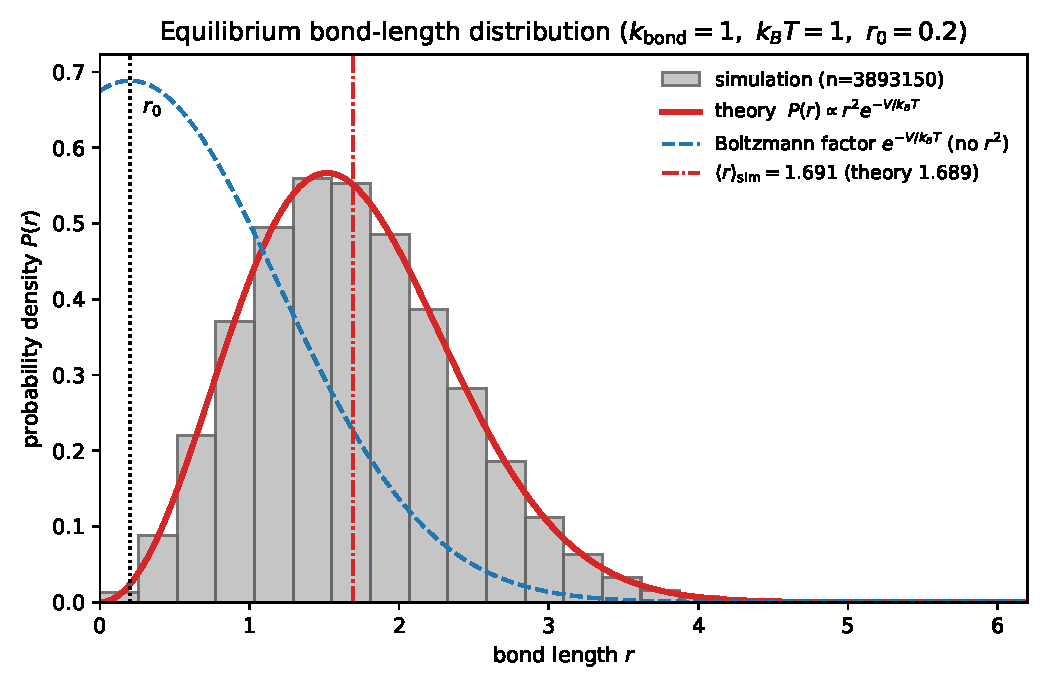
\includegraphics[width=0.86\textwidth]{../figures/bond_length_distribution.pdf}
  \caption{Equilibrium bond--length distribution for $\kbond=\kT=1$, $\rzero=0.2$.
  The measured histogram (grey) from the purely--thermal dumbbell run follows the
  theoretical length pdf $P(r)\propto r^{2}e^{-V/\kT}$ (red), whose mean lies well
  above $\rzero$. The bare Boltzmann factor $e^{-V/\kT}$ without the $r^{2}$ shell
  factor (blue dashed), peaked at $\rzero$, does not describe the data.}
  \label{fig:pdf}
\end{figure}

\begin{table}[h]
  \centering
  \begin{tabular}{@{}lll@{}}
    \toprule
    Dataset & $\avg{r-\rzero}$ & $\avg{r}$ \\
    \midrule
    Simulation (equilibrated, $t\ge1$) & $+1.513\pm0.040$ & $1.713$ \\
    Simulation (all frames)            & $+1.379\pm0.041$ & $1.579$ \\
    Theory, $r^{2}e^{-V/\kT}$          & $+1.490$         & $1.690$ \\
    \bottomrule
  \end{tabular}
  \caption{Mean bond--length deviation from the rest length $\rzero=0.2$ for
  $\kbond=\kT=1$. The equilibrated simulation matches the $r^{2}$--weighted theory
  to within one standard error.}
\end{table}

\section{Summary}

\begin{equation}
  \avg{r}\;\approx\;
  \begin{cases}
    2\sqrt{2/\pi}\,\sigma \approx 1.60\,\sqrt{\kT/\kbond}, & \rzero\ll\sigma
      \quad(\text{entropic / Maxwell}),\\[6pt]
    \rzero+\dfrac{2\kT}{\kbond\,\rzero}, & \rzero\gg\sigma
      \quad(\text{energetic}).
  \end{cases}
\end{equation}
The nonzero mean deviation $\avg{r-\rzero}\approx1.5$ observed in the thermal
dumbbell test is therefore \emph{correct} equilibrium behaviour---an entirely
entropic effect of the $4\pi r^{2}$ shell area---and not a symptom of a spurious
force. The convention--free diagnostic for an unbiased integrator remains the mean
bond \emph{vector} $\avg{\vb{b}}$ and its per--sample increments, both of which
vanish. To make the scalar deviation small one must enter the stiff regime,
$\kbond\rzero^{2}\gg\kT$.

\end{document}
